% Define document class
\documentclass[11pt]{report}
\usepackage{aas_macros}

% Citations
\usepackage{natbib}
\bibliographystyle{abbrvnat}
\setcitestyle{authoryear}

% Language 
\usepackage[utf8x]{inputenc}

% Layout and margins 
\usepackage[margin=1in]{geometry}
\usepackage{layout}
\usepackage{lastpage}
\usepackage{titling}

% Figures & tables 
\usepackage{graphicx,xcolor}
\usepackage{caption}
\usepackage{subcaption}
\usepackage{booktabs} % much better looking tables

% Math 
\usepackage{amsmath,amssymb,bm}
\DeclareMathOperator*{\argmax}{arg\,max}
\usepackage{siunitx} % for proper units 

% Other packages
\usepackage{url}
\usepackage{epstopdf}
\usepackage[font=scriptsize]{caption} % smaller font for fig captions
\usepackage{placeins}
%\usepackage{import}
% of references  

% Settings
\hfuzz=6pt % tolerance on hbox overflows

% Custom command
\newcommand{\ud}{\,\mathrm{d}}
\renewcommand{\vec}[1]{\bm{#1}}

\hypersetup{
    colorlinks=true,
    allcolors=cyan,
}

% Begin!
\begin{document}

% Title
\title{\vspace{-15pt}\begin{center}
\includegraphics[width=0.4\linewidth]{static/misc/logo.jpg}\end{center}
    \vspace{20pt}
    \begin{center}
        School of Physics \& Astronomy
    \end{center}
    \vspace{20pt}
    \begin{center}
        \LARGE\textbf{Probabilistic modeling of astrophysical time series:
            gravitational microlensing and occultation mapping of planets and moons}
    \end{center}
    \vspace{20pt}
    \begin{center}
        Supervisor: Dr. Martin Dominik
    \end{center}
}

\maketitle
\tableofcontents

% Abstract 
\chapter*{Abstract}

Scientific progress in modern astronomy research commonly relies on gathering
large quantities of data using exceedingly precise instruments. The process
which ``generates'' these data consists of the physical phenomenon of interest
-- for instance, an exoplanet blocking or twisting the light of a distant star,
and the noise introduced by the measurement process and the presence of an
atmosphere The task for an astronomer is to first construct a \emph{model}
which describes the entire process which generated the data and to then ``fit''
that model to data. All models only approximate reality and the researcher has
to make a series of decisions during the model building process, everything
from how to process the raw data to which results to put in the abstract of a
paper. Advancements in computational statistics and machine learning in the
past decade or so have made it possible to fit ever more complex models to
data. These models are generally expressed in computer code which may contain
complex numerical algorithms, such as iterative solvers and numerical
integrals. In this thesis, I mostly focused on developing methods which enable
\emph{statistical inference} with these kinds of complex models in two
particular domains within astronomy, gravitational microlensing and occultation
mapping. The common theme between these two topics is that both deal with
accurately measuring the brightness of distant stars as a function of time with
the goal of inferring properties of exoplanets and stars. Broadly speaking, I
believe the biggest contribution of this thesis is providing a new lens for
looking at a particular set of old problems, a lens which incorporates recent
advancements from statistics, machine learning and computer science. More
specifically, I have developed a an open-source software package
\textsf{caustics}\footnote{\url{https://github.com/fbartolic/caustics}} which
enables fast and accurate computation of binary lens and triple lens
microlensing light curves and simultaneously provides exact \emph{gradients} of
the code outputs with respect to all its inputs. This is significant because it
for the first time enables the use of modern gradient based statistical
inference algorithms such as Hamiltonian Monte Carlo with microlensing light
curves. Microlensing is one of the major goals for the upcoming \emph{NASA
    Roman} telescope and the existing modeling methods are completely inadequate
for dealing with the scale of data which will come from \emph{Roman}. I also
propose a framework for dealing with issues which have plagued the field for
decades -- various pathologies in microlensing models and questions about the
interpretation of statistical results. Besides microlensing, I have also delved
into the field of occultation mapping of Solar System objects and exoplanets.
Together with collaborators, I have developed a novel statistical method for
reconstructing spatial maps of volcanic emission on Jupiter's moon Io using
infra-red occultation light curves. I applied the same method to exoplanets to
explore the exciting possibility of detecting weather changes on Hot Jupiters
by reconstructing two dimensional maps of the emission surface from simulated
\emph{JWST} secondary eclipse light curves. I found that planetary scale
changes in the emission pattern should be detectable with \emph{JWST}.

\newpage
\thispagestyle{empty}

% CHAPTER 1: Introduction
\chapter{Introduction}
\section{Context}

The key idea of the scientific revolution in the 16th century was to carefully
observe the world, build \emph{models} which describe some aspect of the
observed phenomenon, and finally and most importantly -- test those models to
see if they provide an accurate description of reality. Since the time of
Galileo, this process gave rise to the modern world and revolutionised our
understanding of the universe. Today we have amazingly accurate models of the
universe. Einstein's theory of \emph{General Relativity} which describes the
universe at a large scale and the \emph{Standard Model} which describes the
universe at the atomic and subatomic scales, both of which were developed in
the 20th century. In my opinion, the two most important questions for the
physical sciences in the 21st century and beyond are the following:
\begin{itemize}
    \item How do we combine the Standard Model and General Relativity to get a complete
          physical theory of the Universe?
    \item What is the origin and distribution of complex life in the Universe?
\end{itemize}

It used to be the case that conducting experiments with the potential to to
change our understanding of fundamental physics was relatively straightforward
and could be conducted by a single person or a small group of researchers. I
have in mind, for instance, Kepler's observations of planetary orbits, Ernest
Rutherford's experiments with atoms or Arthur Eddington's observations of the
Solar eclipse with the goal of testing General Relativity. The data gathering
process consisted of writing notes in a physical notebook and the analysis
hardly required complex statistics. Today the situation is more complicated
because much of the ``low-hanging fruit'' of scientific discovery (in the
physical sciences) has been exhausted and the use of computers is absolutely
central to the process. Progress today usually (but not always) requires
coordination between many scientists, engineers and software engineers building
highly complex experiments. Consider this list of some of the most notable
scientific discoveries in the past few decades:
\begin{itemize}
    \item  Discovery of accelerated expansion of the Universe
    \item  First sequencing of the human genome
    \item  Detection of the Higgs Boson
    \item  Paleogenomics studies of the origin of Homo Sapiens
    \item  Detection of gravitational waves by LIGO
    \item  Reconstruction of the first image of a Black Hole
\end{itemize}
All of these discoveries required gathering substantial amounts of data and the use of
relatively complex statistical analysis techniques.
Computation and statistical analysis are now absolutely central the process of scientific
discovery.

Simultaneously, in the past decade there's been a complete revolution in the
field of machine learning/AI thanks to the advent of deep learning and neural
networks. Besides the incredible progress on predicting patterns in language
and vision, deep learning has also been used in science for things like solving
the protein folding problem \citep{2021Natur.596..583J} and in mathematics for
the purpose of discovering novel conjectures and theorems
\citet{2021Natur.600...70D}. Deep learning has been less useful in physics and
astronomy so far but as I will argue in this thesis, some of the technologies
which underlie deep learning such as automatic differentiation and GPU
computing are going to be (if they aren't already) crucial for processing and
understanding complex datasets in physics and astronomy.

\begin{figure}
    \begin{centering}
        \includegraphics[width=0.8\linewidth]{figures/ads_keyword_bayesian.pdf}
        \caption{Number of NASA/ADS entries containing the keyword ``Bayesian'' per year.}
        \label{fig:ads_keyword_bayesian}
    \end{centering}
\end{figure}

There is another revolution worth mentioning. It is slightly less obvious than
the one in machine learning but nevertheless significant. In the past two
decades there has been a substantial increase in popularity of Bayesian
statistics. Fig~\ref{fig:ads_keyword_bayesian} shows that number of entries in
the NASA/ADS database containing the keyword ``Bayesian'' each year is growing
almost exponentially. One of the reasons that these methods are so popular now
even though they have been invented many decades ago is that they used to be
very computationally expensive and the algorithms necessary to do proper
Bayesian analysis were somewhat underdeveloped. This has changed drastically in
the past decade. I will discuss these methods in detail in
\S~\ref{sec:bayesian_statistics}. Much of this thesis is about applying
Bayesian methods to problems in astronomy.

Having situated the work presented this thesis in the present moment and point
out some scientific and technological changes that I think are relevant, I will
now focus on astronomy in particular. The kinds of questions in astronomy that
most excite me are those which lead us closer to answering one of those two
fundamental questions I stated at the beginning of this chapter. The question
about the origin of life in the universe in particular. Since the first
discoveries of planets outside of our Solar System in the early 90s
\citep{1992Natur.355..145W,1995Natur.378..355M} thousands more have been
confirmed\footnote{At the time of writing the
    \href{https://exoplanetarchive.ipac.caltech.edu/}{NASA Exoplanet Archive}
    contains more than 5000 exoplanets.} using methods such as transits, radial
velocity, microlensing and direct imaging. Thanks to gravitational microlensing
we now know \citep{2012Natur.481..167C} that there is an average one planet per
star in the Milky Way. In addition to detecting the presence of the planets and
inferring their properties such as mass, radius, and orbital period; it is now
possible to measure the transmission and emission spectra of their atmospheres
and even reconstruct crude maps of their surfaces\footnote{The subject of
    Chapter~\ref{ch:mapping_exoplanets}.}
\citep{2007Natur.447..183K,2012ApJ...747L..20M}. With the James Webb Space
Telescope, we might even be able to detect biosignatures in the atmospheres of
Earth size planets.

Answering a grand question such as ``are there biologically produced complex
molecules in this exoplanet atmosphere'' will not be easy even with
cutting-edge instruments such as the James Webb Space Telescope. It will also
almost certainly not be a clear yes or no kind of answer; rather, it will
require a deep understanding (i.e. good \emph{models}) of the physics of
exoplanet atmospheres, stellar variability, the response of the instrument,
sophisticated statistical analysis of the drawing on multiple independent
pieces of evidence and clear definitions of what it means to have detected
something. To build a good model for the thing we really care about requires
understanding also the the things we may intrinsically care less about
(instrumental systematics, details of stellar variability, variations in
Earth's atmosphere etc.).

A large fraction of this thesis (with the exception of
Chapter~\ref{ch:mapping_exoplanets}) is focused on building the necessary
infrastructure (computation, statistics, interpretation) which should enable
new discoveries in exoplanet (and planetary) science. Wherever possible I try
to approach these problems from first principles thinking but with a heavily
computational/statistical approach with a healthy dose of pragmatism. In the
next two sections I will provide a brief introduction to specific areas I
worked on and end the chapter with an outline of the following chapters.

\section{Gravitational microlensing}
\emph{``Do not bodies act upon light at a distance and by their action bend its rays,
    and is not this action strongest at the least distance?''} asked \citet{Newton1704}.
Much later in 1911, even before he published his theory of General Relativity (GR), Einstein
considered the deflection of light from a distant star passing close
to a massive object in the foreground and derived an expression for the deflection angle of the light ray
which was off by a factor of 2 relative to the correct value.
He corrected the error in 1915 using GR.
The first experimental confirmation of this prediction came in 1919 during the
Solar eclipse when the astronomer Arthur Eddington famously measured the
deflection of light from distant stars passing close to the limb of the Sun
\footnote{Weather the data was actually good enough to make the claim that the
    deflection angle is equal to the one Einstein predicted is contested}.
Much later in 1936 a young amateur scientist R.W. Mandl convinced Einstein to
write a short a paper on the lensing effect by a massive star acting as the lens
instead of the Sun.
In the paper \citep{1936Sci....84..506E} Einstein derived an expression for the
magnification of the distant star when it is closely aligned to the foreground lens
star relative to an observer and he predicted that a luminous ring would form
if the two stars were perfectly aligned.
He considered this effect curious but useless, stating that
\emph{``Of course, there is no hope of observing this phenomenon directly.
    First, we shall scarcely ever approach closely enough to such a central line.
    Second, [the angles] will defy the resolving power of our instruments''}.

In this matter, Einstein was wrong. The famous astronomer Fritz Zwicky noticed
the phenomenon is likely to be observable at galactic scales if the lens was a
massive galaxy \citep{1937PhRv...51..290Z,1937PhRv...51..679Z} and that one
could use the measurement of the deflection angle to weigh the lens. Zwicky was
right and the first definitive observation came in 1979 by
\citet{1980ApJ...241..507Y} who observed a double image of the quasar Q0957+561
and concluded that the two images correspond to the same object whose light was
distorted by a massive galaxy. Many other observations followed, including
visible Einstein rings. Far from being just a curious phenomenon, galactic
scale lensing is now one of the key methods of observational cosmology, used
for inferring the parameters of the standard model and the distribution of dark
matter in the universe.

\begin{figure}
    \begin{centering}
        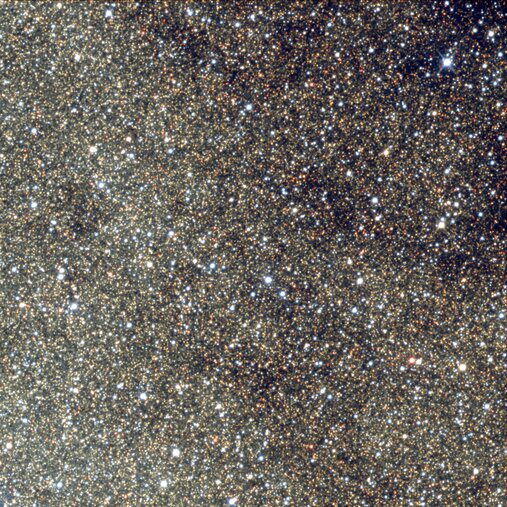
\includegraphics[width=0.5\linewidth]{static/microlensing/crowded_field.jpg}
        \caption{
            Stellar field of a microlensing event GLE-2012-BLG-0406 (centered),
            imaged by one of Las Cumbres Observatory's 2m telescopes,
            showing the high density of stars typical in microlensing observations.
            Credit: Y. Tsapras. Taken from
            \url{http://microlensing-source.org/pictures/}.}
        \label{fig:crowded_field}
    \end{centering}
\end{figure}

That the same effect could be used to detect the presence of planets orbiting
around the lens star was first theorized by \citet{1964PhRv..133..835L} who
wrote that \emph{``the primary effect of planetary deflectors bound to stars
    other than the Sun will be to slightly perturb the lens action of these
    stars''} although he was also sceptical about the possibility of detection,
saying that \emph{``associated pulses would be so weak and infrequent and of
    such fleeting duration – perhaps a few hours – as to defy detection''}.
Gravitational lensing as a method for discovering exoplanets really took off
with the work of Paczyński
\citep{1986ApJ...304....1P,1986ApJ...301..503P,1991ApJ...374L..37M} who also
coined the term \emph{microlensing}, which refers to gravitational lensing in a
regime where the images of the background object cannot be resolved but one can
nevertheless measure its magnification as a function of time. Microlensing as a
method for detecting exoplanets has some unique aspects. First, it is a one-off
event which happens on a timescale of a few minutes up to several months
depending on the distances to the background star and the lensing star and the
mass of the lens. In addition to the fact that there's only one chance to
observe such an event for it to happen at all requires extremely precise
alignment between the lens and the background star and the chance of observing
a stellar microlensing event is about one-in-a-million (CITE) for a typical
star within the Milky Way. To observe a planetary signal is about an order of
magnitude less likely than that. Hence, obtaining a decent sample of planetary
events requires continuous monitoring on the order of $10^{8}$ stars at the
time which way microlensing observations that to focus on the densest region of
the Milky Way -- the galactic bulge. Figure~\ref{fig:crowded_field} a picture
from of such a dense stellar field. Finally, in the vast majority of cases we
do not detect any light from the lens itself, the collected photons are from a
background star completely unrelated and distant from the lensing star. This is
very different from other exoplanet discovery methods and it means that we only
obtain dynamical properties of planets such their masses and periods.

The aspects that make microlensing events that make them difficult to observe
also mean that it provides a unique lens onto exoplanet systems. Relative to
other methods such as transits and radial velocity, microlensing is sensitive
to planets located at substantially greater distances, well outside of our
Solar System neighborhood and even potentially to Milky Way's satellite
galaxies such as the Magellanic Clouds and the nearby Andromeda galaxy (CITE).
Microlensing is also sensitive to very to very small planets and planets which
are further out from the star than those typically detected using transits and
radial velocity. Microlensing surveys such as OGLE \citep{1993AcA....43..289U}
and MOA \citep{1999PThPS.133..233M} have been continuously monitoring crowded
stellar fields in the Milky Way since the 90s\footnote{Initially the focus was
    on finding dark matter candidate particles -- so called MACHOs (Massive Compact
    Halo Objects).} discovering thousands of stellar events and dozens of planetary
events. In order to detect planetary deviations in the observed light curve it
essential to have high cadence observations of the source star. The way surveys
have traditionally worked is that once a particular star started to become
magnified many additional small telescopes would start observing it to obtain
denser coverage and sometimes space-based observatories get involved as well.
The vast majority of microlensing events analyzed so far consist of
observations from multiple observatories, each with its own unique aspects such
as noise properties, cadence and photometric quality.

Future surveys such as the ground based Rubin Observatory
\citep{2019ApJ...873..111I} telescope and the space based Roman Telescope
\citep{2019ApJS..241....3P} and Euclid \citep{2022arXiv220209475B} will detect
tens of thousands of events in total. Although most of past work in the field
focused on characterizing individual events binary lens events, answering
questions about \emph{populations} with these new (but also existing) datasets
requires scalable data analysis methods and algorithms and a clear set of
guidelines on how to interpret the analysis products. This is a substantial
challenge because microlensing events are notoriously difficult to model. Even
though the datasets are relatively simple, consisting of multiple time series
photometric light curves in different bands, the parameter space of even the
simplest models is highly non-linear, correlated, relatively high dimensional
and there are often near perfect degeneracies in the solutions.

The assumptions that existing methods for modeling microlensing events rely on
are often opaque and unquestioned. Discussions on model ``degeneracies''
\citep{2014MNRAS.437.4006S,2019AJ....157...23H,2018AcA....68...43S,2009MNRAS.393..816D},
correlated noise \citep{2015ApJ...812..136B,2019MNRAS.488.3308L} and model
comparison \citep{2018AJ....155..259H,2019MNRAS.484.5608D} have been ongoing in
the microlensing literature for decades without a clear solution and proper
framing of the issue. In this thesis I will revisit these kinds of questions
while taking into account many recent developments in the fields of
computational statistics and machine learning. My main contributions are the
following:
\begin{itemize}
    \item I wrote an open-source Python package \textsf{caustics} which enables fast and
          accurate computation of binary and triple lens microlensing light curves using
          contour integration. The code runs on both CPU and GPU architectures, and
          crucially, for reasons that I will elaborate in subsequent chapters, it
          supports \emph{automatic differentiation} of all outputs with respect to all
          input parameters which enables the use of statistical methods which are orders
          of magnitude more efficient than existing approaches. The code can easily be
          extended to support quadruple lensing and arbitrary intensity profiles for the
          source star.
    \item I have revisited the topic of degeneracies in the posterior probability
          distributions which appear in the context of microlensing and propose solutions
          to these problems.
    \item I have extended the complex polynomial root solver from \citet{Cameron2021}
          such that it can be executed on GPU architectures and that it supports
          automatic differentiation. This enables the evaluation of ~1M lens equation
          solutions for point source binary and triple lenses in seconds using a CPU and
          miliseconds using a GPU.
    \item I propose an approach to statistical inference on a population of microlensing
          events which different from existing methods and has some advantages.
    \item I briefly discuss the issue of correlated noise in microlensing light curves
          and propose ways to account for it using Gaussian Processes.
\end{itemize}

\section{Occultation and phase curve mapping}
Interestingly, the second topic I will cover in this thesis has a history not
unlike that of microlensing. It was proposed in the early 20th century and it
was only much later that technology caught up with the idea. Back in 1906,
\citet{1906ApJ....24....1R} pointed out that certain features in light curves
of Solar System satellites may be attributed to inhomogeneities of their
surfaces. The key idea is that although at any given time we only observe the
total light from an unresolved satellite or planet, different portions of the
surface are visible at different times so we may expect that some of the
information about the surface intensity (be it emission from heat or reflected
Sunlight) gets imprinted onto the light curve. \citet{1906ApJ....24....1R} also
considered the inverse problem -- can we learn something about the surface of
these objects starting from a light curve? The method he proposed is now known
as \emph{phase curve mapping} and it was first attempted by
\citet{1972ApJ...174..449L} who analyzed photometric light curves of Pluto in
reflected light attempting to constrain variations in the \emph{albedo} of the
surface with inconclusive results.

Later works such as
\citet{1992Icar...97..211B,1993Icar..102..134Y,1999AJ....117.1063Y} went a step
further by using not only phase curves but also light curves of mutual
\emph{occultations} of Pluto by its moon Charon to reconstruct albedo maps with
greater success. The major advantage of occultations relative to just phase
curves is that more information about the surface is encoded into the light
curve because of the sharp limb of the occultor sweeping over the disc of an
occulted body and blocking the reflected light. More importantly for this
thesis, \citet{1994Icar..107..195S} was the first to observe the occultations
of Jupiter's moon Io by another of Jupiter's moons -- Europa, and also
occultations of Io by Jupiter itself. These observations were conducted using
near-infrared telescopes such as NASA's Infrared Telescope Facility (IRTF) to
observe emitted light from Io's surface which is covered with many time-varying
and bright volcanic features. The observing campaign of Io has yielded insights
into the the nature of its volcanic activity and it continues to this day. I
will return to the subject of Io in great detail in
Chapter~\ref{ch:mapping_io}.

A natural question arises, can we do this with objects outside of the Solar
System? The answer is yes. \citet{2007Natur.447..183K},
\citet{2012ApJ...747L..20M}, and \citet{arXiv:1202.3829} used Spitzer
mid-infrared observations of secondary eclipses of the Hot Jupiter HD189733b
and found that surface emission is best described by the presence of a large
hot spot on the dayside of the planet which is longitudinally offset from the
substellar point. Similarly, \citet{2014Sci...346..838S}, produced temperature
maps of the Hot Jupiter WASP-43b, \citet{2013ApJ...776L..25D} mapped the Hot
Jupiter Kepler-7b in reflected light and \citet{2016Natur.532..207D} mapped the
thermal emission from the Super Earth 55 Cancri e. These studies were only able
to capture longitudinal variations in intensity. Real exoplanet atmospheres of
are certain to have three-dimensional spatial inhomogeneities in emission more
complex than a single hot spot due to the presence of clouds, zonal jets,
storms, waves etc. \citep{2020SSRv..216..139S}.

In recent years there have been significant advances in statistical modeling of
phase curves and eclipse light curves. Most notably,
\citet{2019AJ....157...64L} introduced the \textsf{starry} code which enables
analytic computation of phase curves and occultation light curves for bodies
with arbitrary emission maps expressed in a spherical harmonic basis (an idea
dating back to \citet{1906ApJ....24....1R} ) and \citet{2021arXiv210306275L}
expanded the algorithm for the (considerably more complicated) case of
reflected light. In this thesis, I will present the work I've done in
collaboration with other researchers from the planetary science and exoplanet
communities on using \textsf{starry} to map the surface of Io and investigate
the prospects for detecting fine spatial structure in the atmospheres of Hot
Jupiters using JWST phase curves and eclipse light curves. My contributions to
this area are the following:
\begin{itemize}
    \item I have developed a novel model for inferring emission maps of Io from
          occultation light curves. First part of this project is published in
          \citet{2022PSJ.....3...67B} though I haven't managed to complete the second
          part.
    \item I have investigated the problem of eclipse mapping of exoplanets using the
          \textsf{starry} framework, focusing in particular on the possibility of
          detecting planetary scale storms on Hot Jupiters using JWST. I found that it
          extremely difficult to infer maps of higher resolution than a dipole order but
          that should still be sufficient for detecting large scale weather and climate
          change in the atmospheres of these planets.
\end{itemize}
The application of the occultation/eclipse mapping method to Io can be seen as the
best case scenario for the application of the same method to exoplanets.
I will show that even in the case of observing a bright object right in our neighborhood,
this is by no means and easy task. Our ability to reconstruct the surface features of
Io sets a sort of upper limit on what is possible with exoplanets.

%\section{Outline}
%The outline of the thesis is as follows. Chapter~\ref{ch:theoretical_min}
%contains the theoretical background needed to understand the subsequent
%chapters, covering the theory behind microlensing and occultation mapping, a
%summary of Bayesian statistics in particular and statistical inference more
%generally, and probabilistic programming which ties everything together.
%Chapter~\ref{ch:microlensing} is the most extensive chapter in the thesis
%covering all of my work on microlensing. I start by discussing the case of
%single lens microlensing models, showing that it contains many of the
%properties of more complex models. In particular I focus on the issue of
%multi-modal posterior distributions which is a ubiquitous problem in
%microlensing. I propose several solutions to this and demonstrate their
%effectiveness. I then move on to the considerably more complex case of binary
%and triple lens models starting with numerical methods for solving the lens
%equation (finding roots of a complex polynomial equation). I demonstrate the
%advantage of the Ehrlich-Aberth algorithm over previous methods and explain how
%to make this algorithm differentiable and orders of magnitude faster through
%the use of GPUs. Next, I cover the contour integration algorithm for computing
%the magnification of a limb-darkened source star and its implementation in
%\textsf{caustics}.

% CHAPTER 2: The theoretical minimum
\chapter{The theoretical minimum}
\label{ch:theoretical_min}

\section{Gravitational microlensing}
\label{sec:microlensing}
\subsection{Deflection of light by gravity}
Gravitational lensing is a phenomenon fully described by Einstein's General
Theory of Relativity (GR) in which light changes its direction of propagation
when passing close to a massive body. GR predicts the following:
\begin{itemize}
    \item the presences of mass changes the spacetime geometry from the flat (Minkowski)
          metric $\eta_{\mu\nu}$ to a curved metric, specified by the tensor $g_{\mu\nu}$
    \item massless particles such as photons follow the null geodesics of the curved
          spacetime which are obtained by solving the \emph{geodesic equation}
\end{itemize}
If we restrict ourselves to the regime where the metric is time independent
and the particles are allowed to travel at any velocity less than $c$,
also known as the \emph{weak field} or \emph{linearized approximation }
of GR, the metric tensor
can be written as
\begin{equation}
    g_{\mu\nu}=\eta_{\mu\nu}+h_{\mu\nu}\quad,
\end{equation}
where $h_{\mu\nu}=
    \textrm{diag}(-2\Phi,-2\Phi,-2\Phi,-2\Phi)$\footnote{Assuming the
    the metric sign convention $(-,+,+,+)$} \citep{carroll_2019}.
The (static) Newtonian gravitational potential $\Phi$ obeys the Poisson equation
\begin{equation}
    \nabla^2\Phi=4\pi G\rho
\end{equation}
where $\rho$ is the mass density of the distribution of mass located between the observer
and the light source.
The geometry of the lensing system consisting of a distant source of light, the
observer, and a distribution of mass with density $\rho$ located between the
source and the observer is shown in Figure~\ref{fig:deflection_angle}.
\begin{figure}
    \centering
    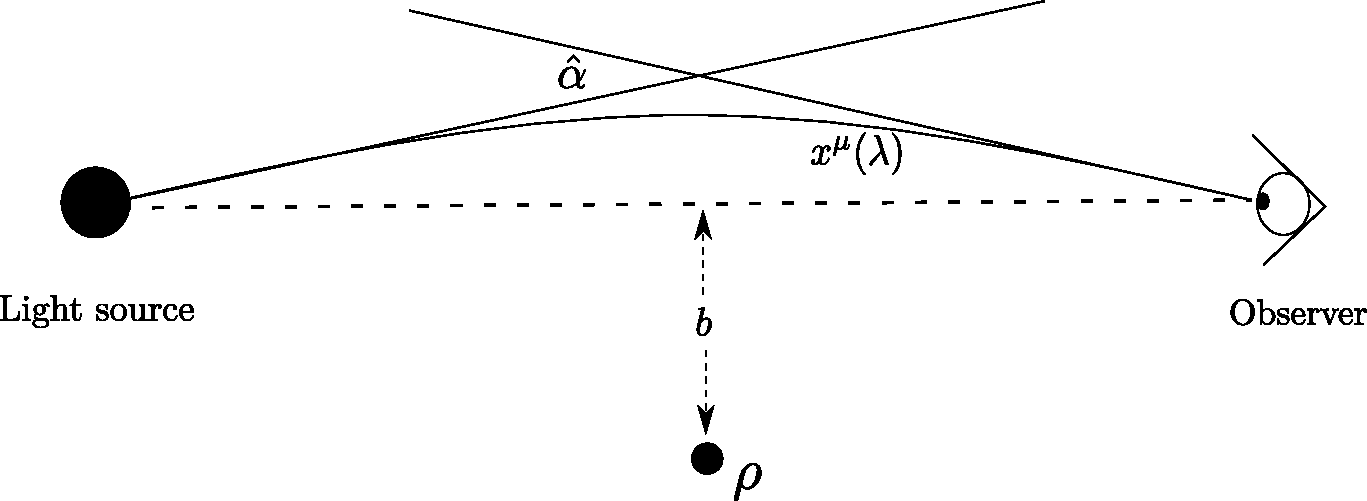
\includegraphics[width=0.6\linewidth]{static/microlensing/deflection_angle.pdf}
    \caption{Geometry of gravitational lensing.
        A geodesic curve $x^\mu(\lambda)$ is deflected
        by an angle $\hat\alpha$ from its initial trajectory
        due to the presence of a massive body with mass density $\rho$. Figure
        adapted from \citet{carroll_2019}.}
    \label{fig:deflection_angle}
\end{figure}
A photon is deflected as it travels from a source to an observer by a
\emph{deflection angle} $\hat\alpha$, a vector in the
plane  perpendicular to the wave vector $\vec{k}$ pointing in the direction of
photon propagation.
The deflection angle is given by \citep{carroll_2019}
\begin{equation}
    \hat\alpha=2\int\nabla_\perp\Phi ds
    \label{eq:deflection_angle_general}
\end{equation}
where $\nabla_\perp\Phi$ is the gradient of the potential in the direction transverse
to the path of the photon and $s$ is the spatial distance traveled.
For a point mass $M$, the potential is given by the potential is
\begin{equation}
    \Phi=- \frac{GM}{(b^2+x^2)^{1/2}}
\end{equation}
where $x$ parametrizes the straight line distance between the observer and the lens and
$b$ is the impact parameter of the light ray.
The deflection angle (in SI units) is then given by
\begin{equation}
    \hat\alpha= \frac{4GM}{c^2b}= \frac{2R_s}{b}
\end{equation}
where the integral has been taken from $-\infty$ to $\infty$ (i.e. assuming that both
the source and the observer are located far away from the deflecting mass) and
$R_s=2GM/c^2$
is the Schwarzschild radius.
The deflection angle $\hat\alpha$ is directly proportional to the mass of the lens and
it does not depend on the wavelength of the light.
It also increases with the proximity of
the light ray to the lensing mass
which is the opposite behaviour to that of a
classical convex lens for which the deflection angle
vanishes at the center of the lens.
The same year Albert Einstein published his General theory of Relativity (1916),
English
physicist Sir Oliver Lodge suggested the light bending phenomenon could produce
a \emph{gravitational lens}.
He warned that it wouldn't be a lens in the usual sense,  because it does not have a
focal length.
In 1936, Einstein showed that a bright background light source perfectly aligned
with a foreground massive body would distort the source in the form of a ring
around the massive body.
However, he concluded that that there is no great chance of discovering such a
phenomenon.
Once astronomers started finding such ring like images in their data the name
\emph{gravitational lensing} caught on.

The resulting deflection angle is very small, for example, for the Sun we have
$GM/c^2=1.48\times 10^5\si{\centi\meter}$ (2.95 km), $R=6.96\times
    10^{10}\si{\centi\meter}$ and $\hat\alpha=1.75$ arc seconds. This deflection
effect was famously claimed to have been observed by Eddington when during a
total solar eclipse in 1919 \citet{2001ASPC..252...21C}, he observed the
position of background stars very close to the Sun's radius in the sky and
compared them to previous measurements taken when the stars weren't close to
the Sun in the sky. He concluded that the observed deflection was in agreement
with GR, although it is doubtful that his data is actually good enough to
distinguish between the GR prediction for the deflection of light and the
Newtonian prediction\footnote{ Gravitational bending on light can be predicted
    in Newtonian mechanics, assuming that light is a massless particle and using
    the equivalence principle which says that that all particles independent of
    their mass accelerate towards massive bodies.} , which is half of the GR value.

It is important to note that Eq.~\ref{eq:deflection_angle_general} is only
valid when the linearized approximation of GR is sufficient. Also, in this
approximation, the deflection angles are additive and the total deflection due
to several massive bodies is just the sum of the individual deflection angles.
The linearized approximation breaks down when the impact parameter $b$
approaches the Schwarzschild radius of the lensing mass and the linearized
metric is no longer sufficient. For most cases of astrophysical interest this
is not an issue.

\subsection{The different scales of lensing}
%% Read the "scales of lensing" paper by that Italian guy
\subsection{Microlensing}
\subsection{The point mass lens and the lens equation}
\subsection{Parallax}
\subsection{Finite source effects}
\subsection{The binary lens}
\subsection{Multiple lenses}
\subsection{Solving the lens equation}

\section{Occultation and phase curve mapping}
\label{sec:occultations}
\subsection{History}
\subsection{The Starry framework}
\subsection{Reflected vs. emitted light}

% In this and the following sections make sure to use microlensing and occultation
% mapping as examples
\section{Bayesian statistics}
\label{sec:bayes}
\subsection{Probability theory}
\subsection{The meaning of probability}
\subsection{Probability as frequency of events in repeated trials}
\subsection{Probability as degrees of belief}
\subsection{The likelihood function}
% mention the likelihood principle
\subsection{Priors}
\subsection{On machine learning and the difference between explanation and prediction}
% mention that even if we have a model focused on inference, it might be best if we judge 
% its quality through its predictive performance

\section{Inference}
\label{sec:inference}
% check that paper on physics and ML by that MIT guy, there's a good stuff there. 
% check also Ian Murray's lecture notes  on MLPR
\subsection{The curse of dimensionality}
\subsection{There's no free lunch}
% exploration vs. explotation 
\subsection{Optimization vs. sampling}
\subsection{Sampling and optimization methods}
\subsubsection{Maximum likelihood}
\subsubsection{The Laplace approximation}
\subsubsection{Variational inference}
\subsubsection{Importance sampling}
\subsubsection{Rejection sampling}
\subsubsection{Markov Chain Monte Carlo}
\subsubsection{Hamiltonian Monte Carlo}
\subsubsection{Other notable methods}

\section{Model validation and comparison}
\label{sec:model_comparison}
\subsection{Cross validation}
% discuss vanilla k-fold CV, stress out just how important and central CV is to science
\subsubsection{Pareto smoothed importance sampling LOO}
\subsection{Model comparison}
% don't do it!

\section{Putting it all together -- \emph{probabilistic programming}}
\label{sec:programming}
\subsection{The success of machine learning}
% that quote from Yann LeCun on differentiable code 
\subsection{Automatic differentiation}
\subsubsection{Forward mode autodiff}
\subsubsection{Reverse mode autodiff or backpropagation}
\subsubsection{Jacobian vector products}
\subsection{JAX}
\subsection{Numpyro}

% CHAPTER 3: Modeling microlensing events 
\chapter{Modeling microlensing events}
\label{ch:microlensing}
\section{Single lens events}
\section{Modeling single lens events}
\section{Numerical solutions to the lens equation}
\section{\textsf{caustics} -- computing the magnification of an extended limb-darkened source}
\section{Comparison with previous work}
\section{Modeling binary lens events}
\section{Population-level inference using hierarchical modeling}

% CHAPTER 4: Mapping the surface of Io 
\chapter{Mapping the surface of Io}
\label{ch:mapping_io}
\section{The data}
\section{Information content}
\section{Pixel sampling}
\section{A static map model}
\section{A dynamic map model}

% CHAPTER 5: Mapping the surfaces of exoplanets
\chapter{Mapping the surfaces of exoplanets}
\label{ch:mapping_exoplanets}
\section{Previous work}
\section{What can we learn using eclipse mapping?}
\section{Time dependent maps}

% CHAPTER 6: Conclusion
\chapter{Conclusion}
\section{Summary of the thesis}
\subsection{Microlensing}
\subsection{Occultation mapping}
\section{Future work}
\subsection{Microlensing in the era of the Roman telescope}
\subsection{Mapping volcanic activity on Io}
\subsection{Mapping exoplanets with JWST and beyond}

\appendix

\chapter{First appendix}
\chapter{Second appendix}

\bibliography{bib.bib}

\end{document}